\header{
    \section{La Strasbourgeoise} \label{la-strasbourgeoise}

    \insertComment{Chant militaire de l'Armée française, aussi connu sous le nom de L'Enfant de Strasbourg, ou encore La Mendiante de Strasbourg.}{Il date de la guerre franco-prussienne de 1870, à la suite de laquelle la France perdit l'Alsace-Lorraine.}
}

\enluminure{4}{\href{}{P}}{etit} papa, c'est donc la mi-Carême,
\\Et te voici déguisé en soldat.
\\Petit papa, dis moi si c'est pour rire,
\\Ou pour faire peur aux tout petits enfants. \bissimple
\\\\Non non ma fille, je pars pour la Patrie,
\\C'est un devoir où tous les papas s'en vont.
\\Embrasse moi petite fille chérie,
\\Je rentrerai bien vite à la maison. \bissimple
\\\\Dis moi maman, quelle est cette médaille,
\\Et cette lettre qu'apporte le facteur ?
\\Dis moi maman, tu pleures et tu défailles,
\\Ils ont tué petit père adoré. \bissimple
\\\\Oui mon enfant, ils ont tué ton père,
\\Pleure avec moi, car nous les haïssons.
\\Quelle guerre atroce qui fait pleurer les mères,
\\Et tue les pères des petits anges blonds. \bissimple
\\\\La neige tombe aux portes de la ville,
\\Là est assise une enfant de Strasbourg.
\\Elle reste là malgré le froid, la bise,
\\Elle reste là malgré le froid du jour. \bissimple
\\\\Un homme passe, à la fillette donne,
\\Elle reconnaît l'uniforme allemand.
\\Elle refuse l'aumône qu'on lui donne,
\\A l'ennemi elle dit bien fièrement : \bissimple
\breakpage
Gardez votre or, je garde ma puissance,
\\Soldat prussien, passez votre chemin.
\\Moi je ne suis qu'une enfant de la France,
\\A l'ennemi je ne tends pas la main. \bissimple
\\\\Tout en priant sous cette cathédrale,
\\Ma mère est morte sous ce porche écroulé.
\\Frappée à mort par l'une de vos balles,
\\Frappée à mort par l'un de vos boulets. \bissimple
\\\\Mon père est mort sur vos champs de bataille,
\\Je n'ai pas vu l'ombre de son cercueil.
\\Frappé à mort par l'une de vos balles,
\\C'est la raison de ma robe de deuil. \bissimple
\\\\Vous avez eu l'Alsace et la Lorraine,
\\Vous avez eu des millions d'étrangers.
\\Vous avez eu Germanie et Bohème,
\\Mais mon p'tit coeur vous ne l'aurez jamais,
\\Car mon p'tit coeur lui restera français!

\\\\
\bigskip
\begin{center}
   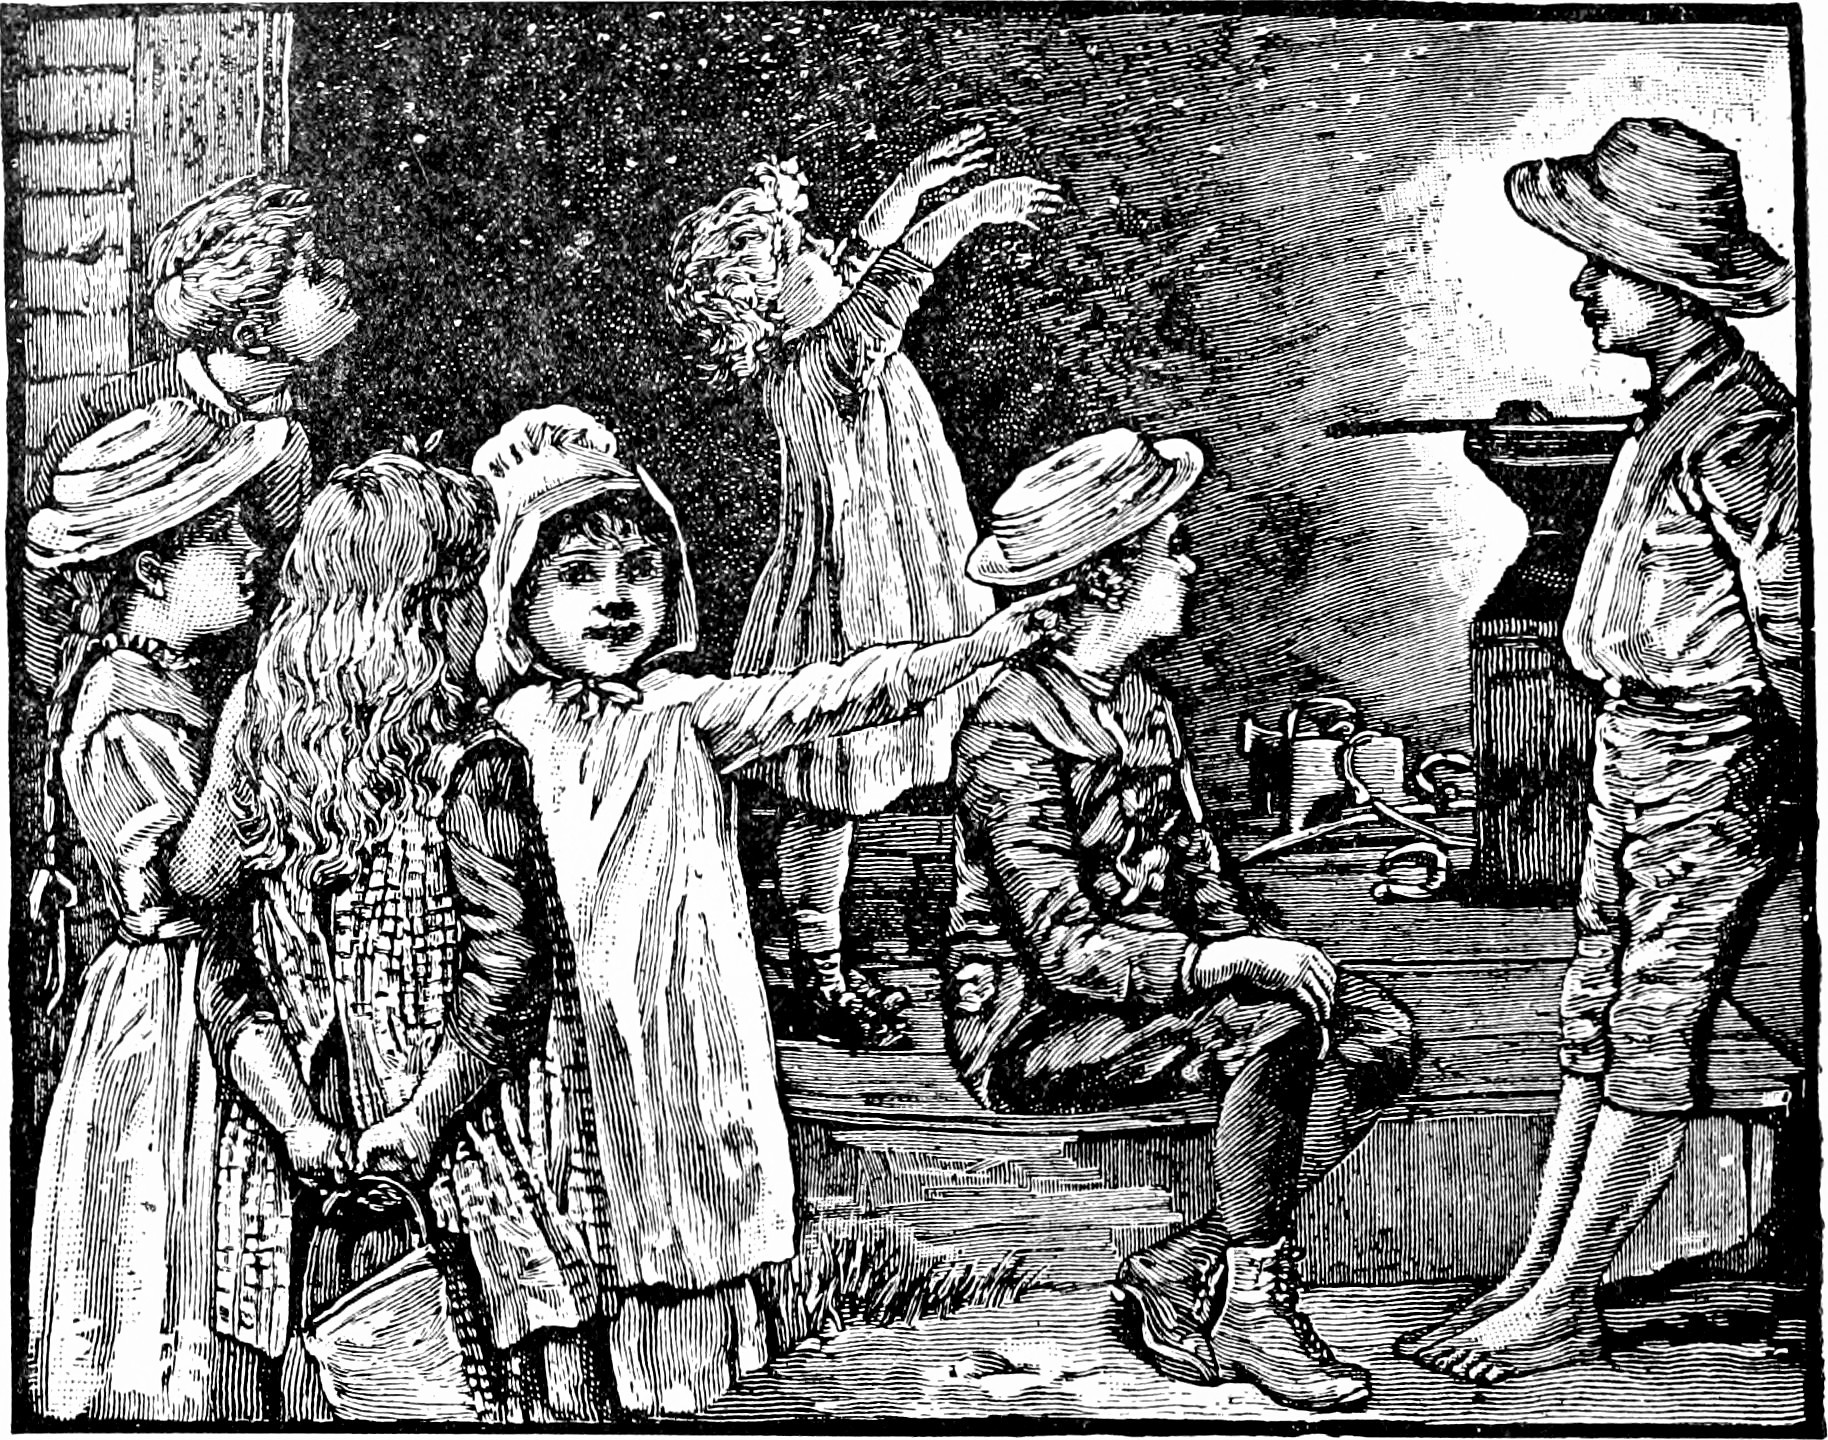
\includegraphics[width=1\textwidth]{images/brev30.png}
 \end{center}

\breakpage